% Chapter Template

\chapter{Methods} % Main chapter title

\label{Chapter2} % Change X to a consecutive number; for referencing this chapter elsewhere, use \ref{ChapterX}

\lhead{Section 2. \emph{Methods}} % Change X to a consecutive number; this is for the header on each page - perhaps a shortened title

%----------------------------------------------------------------------------------------
%	SECTION 1
%----------------------------------------------------------------------------------------

\section{Discrete Framelet Transform}


%-----------------------------------
%	SUBSECTION 1
%-----------------------------------

\subsection{Mallat's algorithm}
The Mallat's algorithm was formally developed in 1988 by Mallat which proves to be a fast algorithm for wavelet decomposition and reconstruction. In the case of discrete wavelet transform, suppose that the length of the signal is $N = 2^J$, the transform can be efficiently computed by implementing Mallat's algorithm with the time complexity $O(N)$. Basically, the algorithm is a classical scheme for deriving the sub-signals using a set of low pass and high pass filters followed by a down-sampling process. To be specific, the low and high pass filters are predetermined by the mother wavelet. Moreover, the low pass filter generates the approximation coefficients and the output of the high pass filters is named detail coefficients. Figure 2.3 and Figure 2.5 shows the diagram of implementing the Mallat's algorithm. After the process of decomposition, the original signal is subsequently decomposed into several sub-signals with different scales.

%-----------------------------------
%	SUBSECTION 2
%-----------------------------------

\subsection{One Level Discrete Framelet Transform}

Equation (1.7) and equation (1.8) indicate that the scaling and wavelet coefficients at level of $j-1$ can be derived from convolving the expansion coefficients at scale $j$ by the coefficients $h_0(-n)$ and $h_1(-n)$ then down-sampling by two, which means taking even terms in the signal sequence and discard the odd terms. Namely, the scale-$j$ coefficients are filtered by two digital filters $h_0(n)$ and $h_1(n)$ and down-sampling the results gives the expansion coefficients at level of $j-1$.(as Figure 2.1 shows)

For the synthesis procedure, it is required to first up-sampling by two and then filtering, where up-sampling by two means inserting zeros between each of the original signal sequence.(as Figure 2.2 shows)
 \begin{figure}[h]
  \centering
  \begin{minipage}[c]{0.5\textwidth}
\centering
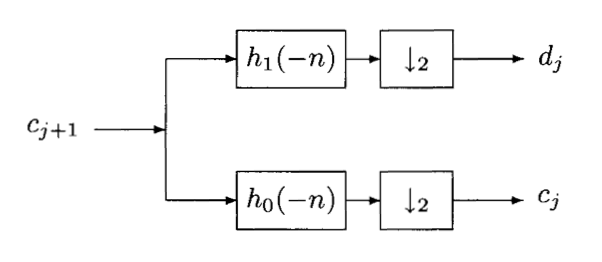
\includegraphics[width=.9\linewidth]{analysis_bank.png}
\caption{One Level Analysis Bank}
\end{minipage}%
%注意这个”%”绝对不能省,可以试试不打%的效果
\begin{minipage}[c]{0.5\textwidth}
\centering
  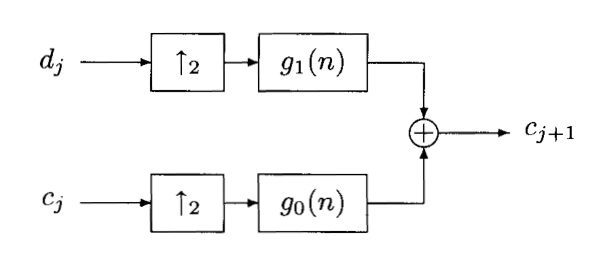
\includegraphics[width=0.9\linewidth]{synthesis_bank.png}
\caption{One Level Synthesis Bank}
  \end{minipage}

\end{figure}


As illustrated in section 1.2, one-level standard discrete framelet transform includes two separate steps named decomposition and reconstruction. Figure 2.3 shows the implementation of one-level discrete framelet transform with a dual framelet filter bank $\{u_0,...,u_s\},\{\tilde{u}_0,...,\tilde{u}_s\}$, the analysis filter $\{u_i\}$ plays the role of filtering the input signal while $\{\tilde{u}_i\}$ is the synthesis filter. The sub-signals are down-sampled after filtered so that the data rates will be the same in the sub-signals as in the original signal. To ease notation, the complex conjugate sequence of u reflected about the origin is denoted as $v^*$, which means $u^*(k) := \overline{u(-k)} $
\begin{figure}[htb]
\centering
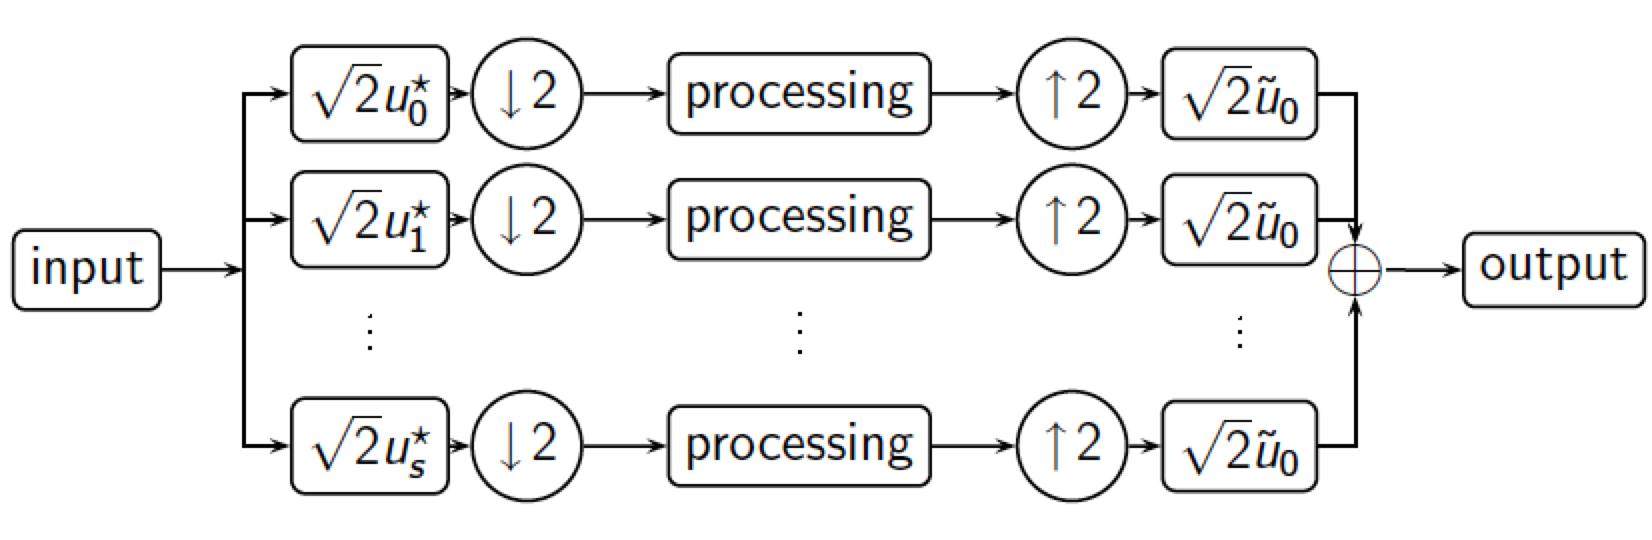
\includegraphics[width=.8\linewidth]{one_level.png}
\caption{Implementation of one-level discrete wavelet transform}
\end{figure}

%-----------------------------------
%	SUBSECTION 3
%-----------------------------------
\subsection{Multi-level discrete wavelet transform}

The filtering and down-sampling procedure can be repeated for several times on the scaling coefficients to give the multi-level structure as illustrated in Figure 2.4. Note that the total number of the sub-signal data will be the same as the number in original data as a result of the down-sampling process. Iterating the filter bank generates more subsets of sub-signals which can be reconstructed through the multi-level synthesis structure later on.
\begin{figure}[htb]
\centering
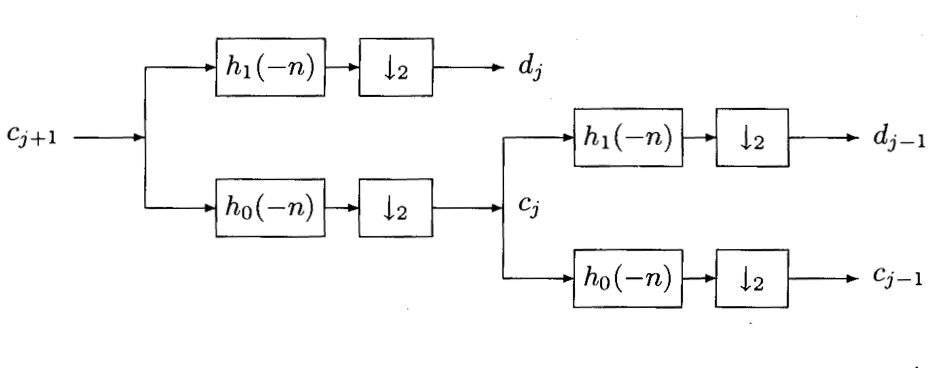
\includegraphics[width=.8\linewidth]{m_analysis_tree}
\caption{Two-level Analysis Tree}
\end{figure}

Figure 2.5 shows the implementation of a two-level discrete framelet transform with a dual framelet filter bank $ \{a,b_1,...,b_s\}, \{\tilde{a},\tilde{b}_1,...,\tilde{a}_s\}$ , also noting the value of the decomposition levels and of the reconstruction levels for a signal should be the same and is particularly determined by the user according to the characters of the original signal and the expected result.

\begin{figure}[htb]
\centering
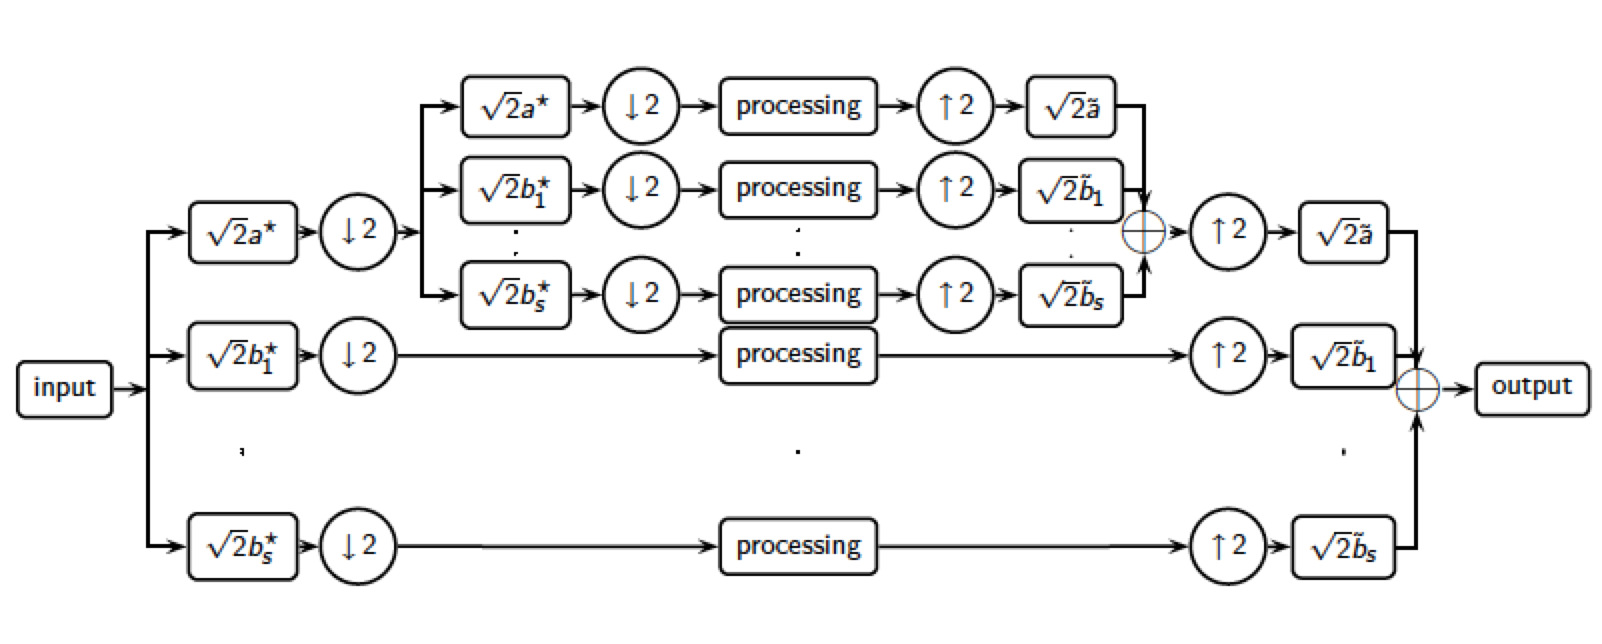
\includegraphics[width=.8\linewidth]{multi_level.png}
\caption{Two-level Discrete Framelet Transform}
\end{figure}


%-----------------------------------
%	SUBSECTION 4
%-----------------------------------

\subsection{Implement the algorithm on Images}
Images is interpreted as a two dimensional matrix with each element representing a pixel in the original image. Therefore, implementing discrete wavelet transform on images requires processing wavelet transform on rows and columns of the 2D matrix. Algorithm 1 briefly illustrates the method for implementing discrete framelet transform on images .


\begin{algorithm}  
\caption{Discrete Framelet Transform on Images}  
\label{alg:1}  
\begin{algorithmic}
\STATE $//$ Transform (Decomposition)
\STATE {parse image signal into a matrix C }
\FOR {each row in C}
\STATE {decompose the row signal according to levels of scale }   
\STATE sort the data into a row and store it into a new matrix D
\ENDFOR
\FOR {each column in C}
\STATE {decompose the column signal according to the same levels of scale}   
\STATE {sort the data into a column and store it into D}   
\ENDFOR
\STATE $//$ Inverse Transform (Reconstruction)
\FOR {each column in D}
\STATE using synthesis bank to reconstruct the column signal from the column in D
\ENDFOR
\FOR {each row in D}
\STATE using synthesis bank to reconstruct the row signal from the row in D
\ENDFOR

\end{algorithmic}  
\end{algorithm}  

Figure 2.6 shows the output of the decomposition process, the sub-bands are organized as rows and columns of the new matrix. With the low pass filter denoted as LP and the high pass filters denoted as HP, it is convenient to denote the output as shown in Figure 2.6. The sub-band $LL_3$ is called the low resolution residual and the others are named details.

\begin{figure}[htb]
\centering
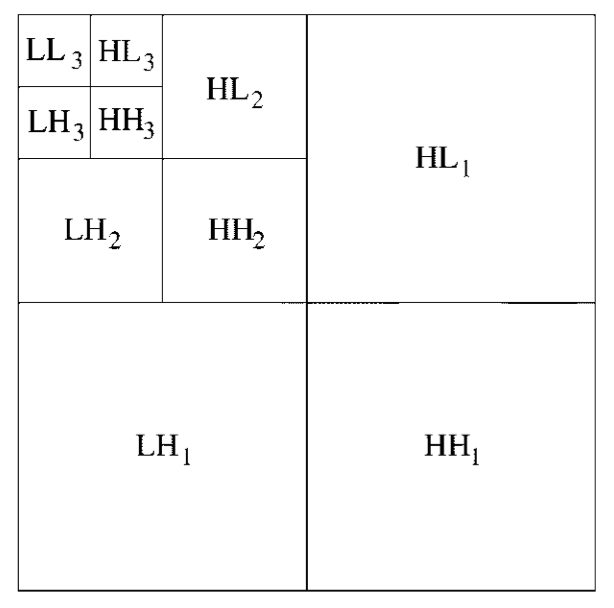
\includegraphics[width=.5\linewidth]{sub_bands.png}
\caption{Sub-bands of the 2D orthogonal wavelet transform}
\end{figure}

%----------------------------------------------------------------------------------------
%	SECTION 2
%----------------------------------------------------------------------------------------

\section{Wavelet Transform in Image Denoising}

It seems often that an image is corrupted by noise when it is transmitted. In that case, the main goal of image denoising is to discard the noise and retain the important signal features as much as possible. Recent work on image denoising through wavelet thresholding has indicated that various wavelet thresholding schemes and different thresholding values for denoising perform well and some of them have near-optimal properties.


\subsection{Problem Formulation}
Assume that there are $n$ noisy samples of function $f(t)$ in total, then denoising problem is usually posed as follows. 
\begin{equation} y_i = f(t_i) + \sigma\varepsilon_i, \qquad i=1,...,n  \end{equation}
Here $\varepsilon_i$ are independent and identically normal distributed $N(0,1)$ and $\sigma$ is called the noise level. As described, our goal is to discard the noise as much as possible and recover the function $f$, where the optimization criterion is the mean squared error (MSE). Namely, it is required to optimize $\hat{f}$ such that $\|\hat f - f\|_2 $ is minimized.

In the 2D scenario, peak signal-to-noise ratio, often abbreviated PSNR, is often used as the optimization criterion. PSNR is directly related to MSE and is defined to be
\begin{equation} PSNR = 10\cdot log_{10}(\frac{MAX^2_I}{MSE})  \end{equation}
where $MAX_I$ is the maximum possible pixel value of the image.

\subsection{Wavelet Thresholding}
Usually the output coefficients of the wavelet transform are sparse, in other words, most values in the coefficients are approximately zero in wavelet transform without the noise. Therefore, in the case of wavelet transform with noise, coefficients with small magnitude are typically noise and ought to be discarded in the denoising problem. The value used to identify noise in this approach is called threshold value and it determines whether a coefficient should be retained. The threshold value denoted by $\lambda$ is usually determined by the decomposition level $j$, e.g. $\lambda= \lambda(j)$

In practice, the thresholding method is only applied to the detail coefficients rather than the approximation coefficients since the approximation coefficients usually contain important components of the signal. Hard thresholding and soft thresholding are often used to thresholding the wavelet coefficients and the rules are given respectively as follows
\begin{eqnarray}
\delta^H_\lambda(d_{jk}) =
\begin{cases}
0       & |d_{jk}|\leqslant \lambda \\
d_{jk}   & |d_{jk}| > \lambda 
\end{cases}
\end{eqnarray}

\begin{eqnarray}
\delta^S_\lambda(d_{jk}) =
\begin{cases}
0       & |d_{jk}|\leqslant \lambda \\
d_{jk}-\lambda   & d_{jk} > \lambda \\
d_{jk}+\lambda   & d_{jk} < -\lambda 
\end{cases}
\end{eqnarray}


\subsection{Algorithm for image denoising}

\renewcommand{\algorithmicrequire}{ \textbf{Input:}} %Use Input in the format of Algorithm  
\renewcommand{\algorithmicensure}{ \textbf{Output:}} %UseOutput in the format of Algorithm  

\begin{algorithm}  
\caption{Image Denoising}  
\label{alg:2}  
\begin{algorithmic}
\REQUIRE ~~\\ %算法的输入参数:Input  
Original Image C; noise level $\sigma$; Decomposition level l; threshold value $\lambda$
\ENSURE ~~\\ %算法的输出:Output  
Image D Recovered from the noise; PSNR value;
\STATE {parse image signal into a matrix C }
\STATE add noise to the image C according to $\sigma$
\FOR {each row in C}
\STATE {decompose the row signal according to l }   
\STATE sort the data into a row and store it into a new matrix D
\ENDFOR
\FOR {each column in C}
\STATE {decompose the column signal according to l}   
\STATE {sort the data into a column and store it into D}   
\ENDFOR
\STATE hard/soft thresholding the matrix D according to $\lambda$
\STATE $//$ Inverse Transform (Reconstruction)
\FOR {each column in D}
\STATE using synthesis bank to reconstruct the column signal from the column in D
\ENDFOR
\FOR {each row in D}
\STATE using synthesis bank to reconstruct the row signal from the row in D
\ENDFOR
\STATE Calculate PSNR for C and D
\end{algorithmic}  
\end{algorithm}  

\begin{figure}[h]
\centering
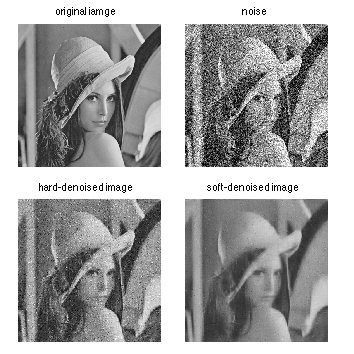
\includegraphics[width=.8\linewidth]{deno_eg.png}
\caption{Image Denoising using hard and soft thresholding with $\sigma = 50$}
\end{figure}



%----------------------------------------------------------------------------------------
%	SECTION 3
%----------------------------------------------------------------------------------------
\newpage
\section{Wavelet Transform in Image Inpainting}

\subsection{Problem Formulation}
Typically, inpainting is described as the way reconstructing deteriorated part of an image. An effective inpainting process involves application of sophisticated algorithms to replace the corrupted part of the image data. Compared to image denoising, a mask matrix representing the corrupted area of the image is required for image inpainting.

Given an image data matrix C and a region $\Omega$ inside it, the inpainting problem consists in reconstructing the data in $\Omega$ in order to eliminate some outstanding difference between the region and its surroundings. A complete process of image inpainting usually requires implementing the wavelet transform recursively for several times in order to reconstruct the image perfectly. Figure 2.8 shows the ouput of the implementation for image inpainting using both hard and soft thresholding.

\subsection{Algorithm for image inpainting}

\renewcommand{\algorithmicrequire}{ \textbf{Input:}} %Use Input in the format of Algorithm  
\renewcommand{\algorithmicensure}{ \textbf{Output:}} %UseOutput in the format of Algorithm  

\begin{algorithm}  
\caption{Image Inpainting}  
\label{alg:3}  
\begin{algorithmic}
\REQUIRE ~~\\ %算法的输入参数:Input  
Original Image C; Mask Matrix M;Recursion times n; Decomposition level l; threshold value $\lambda$
\ENSURE ~~\\ %算法的输出:Output  
Reconstructed Image; PSNR value;
\STATE {parse image signal into a matrix C }
\STATE read a mask M
\STATE C = A.*B is the image with missing information
\FOR {i = 1:n }
\FOR {each row in C}
\STATE {decompose the row signal according to l }   
\STATE sort the data into a row and store it into a new matrix D
\ENDFOR
\FOR {each column in C}
\STATE {decompose the column signal according to l}   
\STATE {sort the data into a column and store it into D}   
\ENDFOR
\STATE hard/soft thresholding the matrix D according to $\lambda$
\STATE $//$ Inverse Transform (Reconstruction)
\FOR {each column in D}
\STATE using synthesis bank to reconstruct the column signal from the column in D
\ENDFOR
\FOR {each row in D}
\STATE using synthesis bank to reconstruct the row signal from the row in D
\ENDFOR
\STATE Update the missing information of C by $C_{new}=(1-M).*D+M.*C$ and replace C by $C_{new}$
\STATE replace threshold value $\lambda$ by a smaller value
\ENDFOR
\STATE Calculate PSNR for C
\end{algorithmic}  
\end{algorithm}  

\begin{figure}[h]
\centering
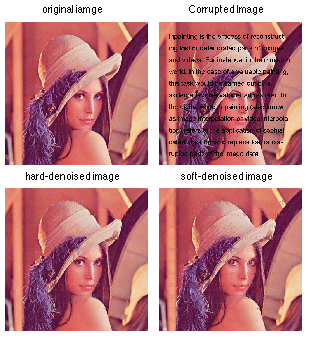
\includegraphics[width=.8\linewidth]{inp_eg.png}
\caption{Image Inpainting using hard and soft thresholding }
\end{figure}

